\documentclass[a4paper,11pt,answers,11pt]{paper}
\usepackage{enumerate}
\usepackage{wrapfig}
\usepackage{fullpage}
\usepackage{textcomp}
\usepackage{charter}
\usepackage[utf8]{inputenc}
\usepackage[T1]{fontenc}
\usepackage{url}
\usepackage{graphicx} % insertion d'images 
\usepackage{hyperref}
\usepackage{lmodern}  % improve pdf rendering
\usepackage{listings} % coloration code
\usepackage{cite}
\usepackage{caption}
\usepackage{upquote}
\usepackage{xcolor}
\usepackage{color}
\usepackage{amssymb,amsmath}
\usepackage{algorithm}
\usepackage{algorithmic}
\usepackage{amsmath}
\bibliographystyle{unsrt}

\lstset{
	language=C++,                   % choose the language of the code
	basicstyle=\footnotesize,       % the size of the fonts that are used for the code
%	numbers=left,                   % where to put the line-numbers
	numberstyle=\footnotesize,      % the size of the fonts that are used for the line-numbers
	stepnumber=1,                   % the step between two line-numbers. If it is 1 each line will be numbered
	numbersep=5pt,                  % how far the line-numbers are from the code
	backgroundcolor=\color{white},  % choose the background color. You must add \usepackage{color}
	showspaces=false,               % show spaces adding particular underscores
	showstringspaces=false,         % underline spaces within strings
	showtabs=false,                 % show tabs within strings adding particular underscores
	frame=single,                   % adds a frame around the code
	tabsize=2,                      % sets default tabsize to 2 spaces
	captionpos=b,                   % sets the caption-position to bottom
	breaklines=true,                % sets automatic line breaking
	breakatwhitespace=false,        % sets if automatic breaks should only happen at whitespace
	escapeinside={\%*}{*)},         % if you want to add a comment within your code
	identifierstyle=\ttfamily,
	keywordstyle=\color[rgb]{0,0,1},
	commentstyle=\color[rgb]{0.133,0.545,0.133},
	stringstyle=\color[rgb]{0.627,0.126,0.941}
}

\definecolor{darkred}{rgb}{0.5,0,0}
\definecolor{darkgreen}{rgb}{0,0.5,0}
\definecolor{darkblue}{rgb}{0,0,0.5}

\hypersetup{
	colorlinks=true,
	%linkcolor=red,%
	linkcolor=darkred,
	filecolor=darkred,
	urlcolor=darkblue,
	citecolor=darkgreen
}

\captionsetup{
  figurename={\sc Fig.},
  tablename={\sc Tab.}
}

% numérotation
\setcounter{tocdepth}{2}    % profondeur 
\setcounter{secnumdepth}{3} % profondeur

% Propriétés doc
\title{$n$-body simulation problem - Gravitation}
\author{Adrien Cassagne}
\date{September 30th 2014}

\begin{document}
\begin{title}
	\noindent\makebox[\textwidth][c]{
		% this is a trick: empty box for avoiding automatic stride in the next includegraphics...
	}
	\noindent\makebox[\textwidth][c]{
		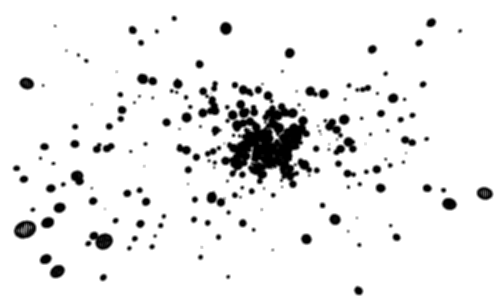
\includegraphics[scale=0.25]{images/nbody.png}
	}
\begin{center}
	{\Large{\texttt{MoveUrBody} code documentation}}\\
\end{center}
\begin{center}
	{\footnotesize{$n$-body problem - Gravity forces}}
\end{center}
\end{title}

\setcounter{page}{1}
\section {Governing equations}
The $n$-body problem is a classic one from the Newtonian mechanics: it consists in resolving the gravity equations.
However, this problem can be generalized (from the algorithmic point of view) and we can often find it in numerical simulation: this is why it is a good real case study.

At the problem beginning (the time $t$), for each body $i$, its position $q_{i}(t)$, its mass $m_i$ and its velocity $\vec{v_i}(t)$ are known.
The applied force between two bodies $i$ and $j$, at the $t$ time, is defined by:
\begin{equation}
\label{eq:force}
	\vec{f_{ij}}(t) = G.\frac{m_i.m_j}{||\vec{r_{ij}}||^2}.\frac{\vec{r_{ij}}}{||\vec{r_{ij}}||},
\end{equation}
with $G$ the gravitational constant ($G = 6,67384\times10^{-11} m^3.kg^{-1}.s^{-2}$) and $\vec{r_{ij}} = q_j(t) - q_i(t)$ the vector from body $i$ to body $j$.
The resulting force (alias the total force) for a given $i$ body, at the $t$ time, is defined by:
\begin{equation}
\label{eq:sumForces}
	\vec{F_i}(t) = \sum_{j \ne i}^{n} \vec{f_{ij}}(t) = G.m_i.\sum_{j \ne i}^{n}\frac{m_j.\vec{r_{ij}}}{||\vec{r_{ij}}||^3},
\end{equation}
with $n$ the number of bodies in space.
For the time integration, the acceleration is required. For a given body $i$, at the $t$ time, the acceleration characteristic is defined by:
\begin{equation}
\label{eq:acceleration}
	\vec{a_i}(t) = \frac{\vec{F_i}(t)}{m_i} = G.\sum_{j \ne i}^{n}\frac{m_j.\vec{r_{ij}}}{||\vec{r_{ij}}||^3}.
\end{equation}

\subsection{An approximation of the total force}

The total force $\vec{F_i}$ is given by Eq.~\ref{eq:sumForces}:
\begin{equation*}
	\vec{F_i}(t) = G.m_i.\sum_{j \ne i}^{n}\frac{m_j.\vec{r_{ij}}}{||\vec{r_{ij}}||^3}.
\end{equation*}
As bodies approach each other, the force between them grows without bound, which is an undesirable situation for numerical integration. 
In astrophysical simulations, collisions between bodies are generally precluded; this is reasonable if the bodies represent galaxies that may pass right through each other. 
Therefore, a softening factor $\epsilon^2 > 0$ is added, and the denominator is rewritten as follows:
\begin{equation}
\label{eq:sumForcesSoft}
	\vec{F_i}(t) \approx G.m_i.\sum_{j = 1}^{n}\frac{m_j.\vec{r_{ij}}}{(||\vec{r_{ij}}||^2 + \epsilon^2)^\frac{3}{2}}.
\end{equation}

Note the condition $j\ne i$ is no longer needed in the sum, because $\vec{f_{ii}} = 0$ when $\epsilon ^2 > 0$.
The softening factor models the interaction between two Plummer point masses: masses that behave as if they were spherical galaxies.
In effect, the softening factor limits the magnitude of the force between the bodies, which is desirable for numerical integration of the system state.

As before, we need to compute the acceleration in order to perform the integration over the time:
\begin{equation}
\label{eq:accelerationSoft}
	\vec{a_i}(t) = \frac{\vec{F_i}(t)}{m_i} \approx G.\sum_{j = 1}^{n}\frac{m_j.\vec{r_{ij}}}{(||\vec{r_{ij}}||^2 + \epsilon^2)^\frac{3}{2}}.
\end{equation}

\section {Collisions}
In \texttt{MoveUrBody} code there is various implementations: some of them are based on colliding bodies.
In this section we try to explain what kind of collisions are used if the implementation considers colliding bodies.

\subsection{Collisions detection}
We choose \textit{a posteriori} method in order to detect collisions: this is a discrete and easy to implement method.
We detect the collisions after they append. 
This is less expensive in term of computations than \textit{a priori} method (continuous).
In \texttt{MoveUrBody} we consider that the shape of all the bodies is a sphere, so two bodies $i$ and $j$ are colliding if:
\begin{equation}	
\label{eq:collsDetection}
	||\vec{r_{ij}}|| - (r_i + r_j) \leq 0,
\end{equation}
where $r_i$ and $r_j$ are respectively the radii of body $i$ and body $j$.

\subsection{Elastic collisions}
Notation: Throughout this section, $m$ is mass and $v$ is velocity.
Be aware that $v = ||\vec{v}||$.
Subscripts $i$ and $j$ distinguish between the two colliding bodies. 
An apostrophe after a variable means that the value is taken after the collision (called prime; i.e., $v$' is "$v$ prime").\\

In \texttt{MoveUrBody} we consider that all collisions are perfectly elastic.
An elastic collision is a collision in which kinetic energy is conserved. 
That means no energy is lost as heat or sound during the collision. 
In the real world, there are no perfectly elastic collisions on an everyday scale of size. 
But you can get the sense of an elastic collision by imagining a perfect pool ball which doesn't waste any energy when it collides. 
In an elastic collision, both kinetic energy and momentum are conserved (the total before and after the collision remains the same).
Momentum is the product of mass and velocity: 
\begin{equation}	
\label{eq:momentum}
	\vec{p} = m . \vec{v}.
\end{equation}
The kinetic energy of an object is one-half times its mass times the square of its velocity:
\begin{equation}	
\label{eq:kinetic}
	E_k = \frac{1}{2} . m . v^2.
\end{equation}
Now it is easy to write the conservation of momentum and kinetic energy as two equations:
\begin{enumerate}
	\item Conservation of momentum
		\begin{equation}	
		\label{eq:momentumCons}
			m_i . \vec{v_i} + m_j . \vec{v_j} = m_i . \vec{v'_i} + m_j . \vec{v'_j}
		\end{equation}
		
	\item Conservation of kinetic energy
		\begin{equation}	
		\label{eq:kineticCons}
			\frac{1}{2} . m_i . (v_i)^2 + \frac{1}{2} . m_j . (v_j)^2 = \frac{1}{2} . m_i . (v'_i)^2 + \frac{1}{2} . m_j . (v'_j)^2
		\end{equation}
\end{enumerate}

\subsubsection{1-Dimensional elastic collisions}
Combining the two previous equations (Eq.~\ref{eq:momentumCons} and \ref{eq:kineticCons}) and doing a lot of algebra gives the final (after collision) velocities of body $i$ and $j$:
\begin{equation}	
\label{eq:1DelasticSols}
	v'_i = \frac{v_i(m_i-m_j) + 2.m_j.v_j}{m_i + m_j},~~v'_j = \frac{v_j(m_j-m_i) + 2.m_i.v_i}{m_j + m_i}.
\end{equation}
This result allows us to find the velocity of two objects after undergoing a one-dimensional elastic collision. 
We will use this result later in the 3-dimensional case.

\subsubsection{3-Dimensional elastic collisions}
In previous sub-section (1D elastic collisions) the vectors representation was not very important.
Now in 3D, we will use the component representation of a vector: $\vec{v} = \left\{ v_x, v_y, v_z \right\}$.\\

We will follow a 7-step process to find the new velocities of two objects after a collision. 
The basic goal of the process is to project the velocity vectors of the two objects onto the vectors which are normal (perpendicular) and tangent to the plan of the collision. 
This gives us a normal component and two tangential components (defining a plan) for each velocity. 
The tangential components of the velocities are not changed by the collision because there is no force along the plan tangent to the collision surface. 
The normal components of the velocities undergo a one-dimensional collision, which can be computed using the one-dimensional collision formulas presented above.
Next the unit normal vector is multiplied by the scalar (plain number, not a vector) normal velocity after the collision to get a vector which has a direction normal to the collision surface and a magnitude which is the normal component of the velocity after the collision. 
The same is done with the unit tangent vectors and the tangential velocity components. 
Finally the new velocity vectors are found by adding the normal velocity and the two tangential velocity vectors for each object.

\paragraph{Step 1}
~\\
Find the unit normal and the two unit tangent vectors.
The unit normal vector is a vector which has a magnitude of 1 and a direction that is normal (perpendicular) to the surfaces of the objects at the point of collision. 
The two unit tangent vectors are vectors with a magnitude of 1 which are forming a tangent plan to the circle's surfaces at the point of collision.
	
First find a normal vector.
This is done by taking a vector whose components are the difference between the coordinates of the centers of the spheres. 
Let $q_i = \left\{q_{ix}, q_{iy}, q_{iz}\right\}$, $q_j = \left\{q_{jx}, q_{jy}, q_{jz}\right\}$ coordinates of the centers of the spheres (it does not matter which spheres is labelled $i$ or $j$; the end result will be the same).
Then the normal vector $\vec{n}$ is: 
\begin{equation*}	
	\vec{n} = \left\{ q_{jx} - q_{ix},~q_{jy} - q_{iy},~q_{jz} - q_{iz}  \right\}.
\end{equation*}
Next, we have to find the unit vector of $\vec{n}$, which we will call $\vec{un}$. This is done by dividing by the magnitude of $\vec{n}$:
\begin{equation*}	
	\vec{un} = \frac{\vec{n}}{||\vec{n}||} = \frac{\vec{n}}{\sqrt{n_x^2 + n_y^2 + n_z^2}}.
\end{equation*}
Once it's done we need to find the two unit tangent vector which are forming the collision tangent plan.
Those two unit tangent vectors ($\vec{ut_1}$ and $\vec{ut_2}$) are perpendicular to the unit normal vector $\vec{un}$ and there are also perpendicular between themselves (in order to form a Cartesian coordinate system).
Before trying to determine two unit tangent vectors $\vec{ut_1}$ and $\vec{ut_2}$ we will try to find two tangent vectors $\vec{t_1}$ and $\vec{t_2}$.
If $\vec{t_1}$ is perpendicular to $\vec{un}$ then the scalar product of the two should be null:
\begin{equation*}
	\vec{t_1} . \vec{un} = 0 \Leftrightarrow	(t_{1x} . un_x) + (t_{1y} . un_y) + (t_{1z} . un_z) = 0.
\end{equation*}
The first and easy solution to this previous equation is the null vector $\vec{0}$ but we obviously want to avoid it.
An idea is to fix one of the three components to 0 and an other to 1 in order to determine a perpendicular vector $\vec{t_1}$ (be aware that there is an infinity of perpendicular vectors to $\vec{un}$ and we just need to find one of them).\\
If $un_x \neq 0$:
\begin{equation*}
	\vec{t_1} = \left\{ -\frac{un_y}{un_x}, 1, 0 \right\}.
\end{equation*}
If $un_y \neq 0$:
\begin{equation*}
	\vec{t_1} = \left\{ 1, -\frac{un_x}{un_y}, 0 \right\}.
\end{equation*}
If $un_z \neq 0$:
\begin{equation*}
	\vec{t_1} = \left\{ 1, 0, -\frac{un_x}{un_z} \right\}.
\end{equation*}
We have to choose one of the three previous propositions and be sure to avoid to divide by 0.
Now we have to normalize $\vec{t_1}$ in order to find the unitary $\vec{ut_1}$ vector:
\begin{equation*}
	\vec{ut_1} = \frac{\vec{t_1}}{||\vec{t_1}||} = \frac{\vec{t_1}}{\sqrt{t_{1x}^2 + t_{1y}^2 + t_{1z}^2}}.
\end{equation*}
It remains to determine the $\vec{ut_2}$ vector, this can be done by computing the cross product between $\vec{un}$ and $\vec{ut_1}$:
\begin{equation*}
	\vec{ut_2} = \vec{un} \wedge \vec{ut_1} = \left\{ (un_y . ut_{1z} - un_z . ut_{1y}), (un_z . ut_{1x} - un_x . ut_{1z}), (un_x . ut_{1y} - un_y . ut_{1x})\right\}.
\end{equation*}

\paragraph{Step 2}
~\\
Create the initial (before the collision) velocity vectors, $\vec{v_i}$ and $\vec{v_j}$. 
These are just the $x$, $y$ and $z$ components of the velocities put into vectors: $\vec{v_i} = \left\{ v_{ix}, v_{iy} \right\}$ (and similarly for $\vec{v_j}$). 
Note that this step really isn't necessary if the velocities are already represented as vectors. 
This step is needed only if the velocities are initially represented as separate $x$, $y$ and $z$ values.

\paragraph{Step 3}
~\\
Keep in mind that after the collision the tangential components of the velocities are unchanged and the normal component of the velocities can be found using the one-dimensional collision formulas presented earlier. 
So we need to resolve the velocity vectors, $\vec{v_i}$ and $\vec{v_j}$, into normal and tangential components. 
To do this, project the velocity vectors onto the unit normal and unit tangent vectors by computing the dot product. Let $v_{in}$ be the scalar (plain number, not a vector) velocity of body $i$ in the normal direction. 
Let $v_{it1}$ and $v_{it2}$ be the scalar velocity of body $i$ in the tangential directions. 
Similarly, let $v_{jn}$, $v_{jt1}$ and $v_{jt2}$ be for body $j$. 
These values are found by projecting the velocity vectors onto the unit normal and unit tangent vectors, which is done by taking the dot (alias scalar) product:
\begin{equation*}
	v_{in} = \vec{v_i}.\vec{un},~~v_{it1} = \vec{v_i}.\vec{ut_1},~~v_{it2} = \vec{v_i}.\vec{ut_2},
\end{equation*}
\begin{equation*}
	v_{jn} = \vec{v_j}.\vec{un},~~v_{jt1} = \vec{v_j}.\vec{ut_1},~~v_{jt2} = \vec{v_j}.\vec{ut_2}.
\end{equation*}

\paragraph{Step 4}
~\\
Find the new tangential velocities (after the collision). 
This is the simplest step of all. 
The tangential components of the velocity do not change after the collision because there is no force between the circles in the tangential direction during the collision. 
So, the new tangential velocities are simply equal to the old ones:
\begin{equation*}
	v'_{it1} = v_{it1},~~v'_{it2} = v_{it2},
\end{equation*}
\begin{equation*}
	v'_{jt1} = v_{jt1},~~v'_{jt2} = v_{jt2}.
\end{equation*}

\paragraph{Step 5}
~\\
Find the new normal velocities. This is where we use the one-dimensional collision formulas (Eq.~\ref{eq:1DelasticSols}).
The velocities of the two circles along the normal direction are perpendicular to the surfaces
of the circles at the point of collision, so this really is a one-dimensional collision:
\begin{equation*}
	v'_{in} = \frac{v_{in}(m_i-m_j) + 2.m_j.v_{jn}}{m_i + m_j},
\end{equation*}
\begin{equation*}
	v'_{jn} = \frac{v_{jn}(m_j-m_i) + 2.m_i.v_{in}}{m_j + m_i}.
\end{equation*}

\paragraph{Step 6}
~\\
Convert the scalar normal and tangential velocities into vectors. 
This is easy just multiply the unit normal vector by the scalar normal velocity and you get a vector which has a direction that is normal to the surfaces at the point of collision and which has a magnitude equal to the normal component of the velocity. 
It is similar for the tangential components:
\begin{equation*}
	\vec{v'_{in}} = v'_{in} . \vec{un},~~\vec{v'_{it1}} = v'_{it1} . \vec{ut_1},~~\vec{v'_{it2}} = v'_{it2} . \vec{ut_2},
\end{equation*}
\begin{equation*}
	\vec{v'_{jn}} = v'_{jn} . \vec{un},~~\vec{v'_{jt1}} = v'_{jt1} . \vec{ut_1},~~\vec{v'_{jt2}} = v'_{jt2} . \vec{ut_2}.
\end{equation*}

\paragraph{Step 7}
~\\
Find the final velocity vectors by adding the normal and tangential components for each body:
\begin{equation*}
	\vec{v'_i} = \vec{v'_{in}} + \vec{v'_{it1}} + \vec{v'_{it2}},
\end{equation*}
\begin{equation*}
	\vec{v'_j} = \vec{v'_{jn}} + \vec{v'_{jt1}} + \vec{v'_{jt2}}.
\end{equation*}
Now we have the final (after collision) velocity of each body as a vector.

\newpage
\section {Time}
\subsection{Time step selection}
The easier way to determine $\Delta t$ is to select it as a constant for all the simulation iterations.
For visualization concerns we will sometimes use a constant $\Delta t$ but, for simulation precision interests, it is better to compute a new time step for each iterations depending on the distance between the nearest bodies.
The following equation describes the variable $\Delta t$ calculation:
\begin{equation}
\label{eq:dt1}
	\|\vec{v_i}(t) . \Delta t + \frac{\vec{a_i}(t)}{2} . \Delta t^2 \| \leq 0.1 \times ||\vec{r_{ij}}||,
\end{equation}
with $j$ the nearest body to the body $i$.
For each body $i$, a time step is calculated and the smallest one is chosen.
Eq.~\ref{eq:dt1} traduces that the distance between $i(t)$ and $i(t + \Delta t)$ must be below 10\% of the $||\vec{r_{ij}}||$ distance.
This equation assures that two masses cannot be closest than 20\% between $t$ time and $t + \Delta t$ time.
However, Eq.~\ref{eq:dt1} is not directly usable: this is a $4^{th}$ degree polynomial equation in $\Delta t$.
It's why we will use the triangle inequality witch allows us to determine a new condition:
\begin{equation}
\label{eq:dt2}
	\|\vec{v_i}(t)\| . \Delta t + \frac{\|\vec{a_i}(t)\|}{2} . \Delta t^2  \leq 0.1 \times ||\vec{r_{ij}}||.
\end{equation}
Eq.~\ref{eq:dt2} is a $2^{nd}$ degree equation: this is more reasonable in term of computational time.

\subsection{Time integration}
The integrator used to update the positions and velocities is a leapfrog-Verlet integrator (Verlet 1967) because it is applicable to this problem and is computationally efficient (it has a high ratio of accuracy to computational cost).

Body $i$ velocity characteristic at the $t + \Delta t$ time depends on the velocity and the acceleration at the $t$ time:
\begin{equation}
\label{eq:velocity}
	\vec{v_i}(t + \Delta t) = \vec{v_{i}}(t) + \vec{a_i}(t) . \Delta t.
\end{equation}
At the end, body $i$ position $q_i$ at the $t + \Delta t$ time depends on the position, the velocity and the acceleration at the $t$ time:
\begin{equation}
\label{eq:position}
	q_i(t + \Delta t) = q_{i}(t) + \vec{v_{i}}(t) . \Delta t + \frac{\vec{a_i}(t) . \Delta t^2}{2}.
\end{equation}
Thanks to Eq.~\ref{eq:acceleration}, \ref{eq:velocity} and \ref{eq:position}, it is now possible to compute the new position and the new velocity for all bodies at the $t + \Delta t$ time.


\newpage
\section {Implementations}
\subsection{Algorithmic}
From an algorithmic point of view, we are calculating each body depending on all the other bodies.
We can traduce that by 2 overlapping \texttt{for-loops} from $0$ to $n$ bodies. 
In a \texttt{C-like} language we can express the problem this way:
\begin{lstlisting}[caption={$n$-body pseudo-code algorithm},label={alg:ncorps}]
body b1[N]; // array which contains all the bodies (at t time)
body b2[N]; // empty array
for(unsigned int iBody = 0; iBody < n; ++iBody)
	for(unsigned int jBody = 0; jBody < n; ++jBody)
		if(iBody != jBody)
			b2[iBody] = compute(b1[jBody]);
\end{lstlisting}
Alg. \ref{alg:ncorps} shows an important characteristic of the $n$-body problem class: for $n$ given bodies, the algorithmic complexity in term of computational time is approximatively $O(n^2)$.
It exists other methods to approximate and to resolve the problem in $O(n \log{n} )$ time but this is not in the range of this lab (see {\sc Barnes-Hut} simulation).

\newpage
\section {Code compiling and code execution}
\subsection{Compile the executable}

For some practical reasons the project use \texttt{cmake} instead of a standard \texttt{Makefile}.
Don't panic this is not very complicated and this section is made to help you.
First thing to do is to generate the \texttt{Makefile} with the \texttt{cmake} system:
\begin{lstlisting}[language=c]
> cmake .
\end{lstlisting}
This command will generate the \texttt{Makefile} file in the current directory.
But before using the \texttt{Makefile} we will configure the generated \texttt{CMakeCache.txt} file.
This file is the configuration file for specify our favourite compiling options.
Here is the recommended configuration:
\begin{lstlisting}[language=c]
//Choose the type of build, options are: None(CMAKE_CXX_FLAGS or
// CMAKE_C_FLAGS used) Debug Release RelWithDebInfo MinSizeRel.
CMAKE_BUILD_TYPE:STRING=Release

//Flags used by the compiler during all build types.
CMAKE_CXX_FLAGS:STRING=-DNBODY_FLOAT -march=native -fopenmp
\end{lstlisting}
Now we can use the \texttt{Makefile} with this command:
\begin{lstlisting}[language=c]
> make
\end{lstlisting}
After that, the binary file will be generated in \texttt{bin/Release/nbody}.
Launch the executable like this from the root folder:
\begin{lstlisting}[language=c]
> ./bin/Release/nbody
\end{lstlisting}

\subsection{Run the executable}

There is two ways to launch the initial $n$-body code.
The first one initializes bodies from an input file:
\begin{lstlisting}[language=c]
Usage: ./bin/Release/nbody -f inputFile -i nIte [-h] [-v] [-w outputFiles]

	-f		the bodies input file name to read.
	-i		the number of iterations to compute.
	-h		display this help.
	-v		enable the verbose mode.
	-w		the base name of the body file(s) to write.
\end{lstlisting}
The \texttt{data/in} folder contains some test cases, you can launch them like this:
\begin{lstlisting}[language=c]
> ./bin/Release/nbody -f data/in/8bodies.dat -i 200 -w data/out/8bodies
\end{lstlisting}
This command will run the 8bodies test case with 200 iterations and will write the solution at each iteration in \texttt{data/out/8bodies.*.dat} files.

There is not big enough test cases to really fill the CPU capacity. 
This is why there is an other way to launch the $n$-body code based on the number of bodies we want to simulate:
\begin{lstlisting}[language=c]
Usage: ./bin/Release/nbody -n nBodies -i nIte [-h] [-v] [-w outputFiles]

	-n		the number of bodies randomly generated.
	-i		the number of iterations to compute.
	-h		display this help.
	-v		enable the verbose mode.
	-w		the base name of the body file(s) to write.
\end{lstlisting}
You can launch the $n$-body code like this:
\begin{lstlisting}[language=c]
> ./bin/Release/nbody -n 500 -i 1000 -v
\end{lstlisting}
This command will launch the simulation with 500 bodies randomly generated (1000 iterations). Note that the verbose mode is enabled, so it will display some information for each iteration in your shell.

There is a lot of other options you can use with this code: try the \texttt{-h} option to display them.
If you do not want to run OpenGL rendering you can put the \texttt{-\--nv} (no visualization) in order to disable it.

\end{document}
